\setstretch{1.5}
\chapter{Protocol}
\section{Introduction}
\subsection{Background}
Idiopathic Parkinson's disease (\acs{iPD})\acused{iPD} represents a chronic neurodegenerative disorder manifested by both motor and non-motor symptoms. The physical impairments in \ac{iPD} have a significant psychosocial impact and lead to considerable losses in patients'  \ac{QoL} and a high burden on (informal) caregivers. Several \ac{QoL} assessment tools have been developed so far, some of which are specific to \ac{iPD} \cite{stuhrenberg2022jpm}. However, none of the models take into account positive aspects of well-being or a subject's personal attitude (e.g., optimism) but also manifold aspects in someone's life such as lack of social support as possible stress factor or level of integration, to name a few.

This project will investigate the \ac{QoL} of patients with \ac{iPD} over time. To this end, a longitudinal assessment will be carried out using established and validated \ac{HRQOL} questionnaires. In addition, holistic observations will be collected using a model developed from the \textsc{CHAPO} model \citep{thieken2022jpd} -- an approach originally developed to assess quality of life in very old people\footnote{\url{https://ceres.uni-koeln.de/forschung/nrw80}}. This approach has been refined and adapted to aspects of \ac{iPD} patients for this cohort study. The aim of this project is therefore to record \ac{QoL} in a standardised way over a long period of time. These data will also be correlated with biomarkers obtained annually in the form of a cranial \ac{MRI} and blood, saliva, urine, hair and stool samples. We aim to identify biomedical markers with predictive value for changes in \ac{QoL}. In addition, the approach in this longitudinal study also aims to identify the support services needed to better meet the needs of family members of \ac{iPD} patients. Carers' experience of stress, changes in sleep patterns and loss of \ac{QoL} over the observation period will be included in the analysis to identify a proxy for adequate support.

\subsection{Geographic context}
\ac{iPD} is one of the most common neurological disorders. Estimates put the incidence of the disease in Germany at \SI{84.1}{} per \num[round-precision = 0, round-mode = places]{100000}{} people per year and assume a number of \num[round-precision = 0, round-mode = places]{400000}{} people \citep{nerius2017parkinson}. In order to understand the particularities of the \UKM as far as the care of \ac{iPD} patients is concerned, it is necessary to know the location of Marburg. About \SI[round-precision = 0, round-mode=places]{77000}{} people live in the city of Marburg, which is located in the countryside of central Germany. It is a university town and a district town in the federal state of Hesse (see figure \ref{fig1:hesseGermany}). Due to its location at about \SI{80}{\km} direct distance between the metropolitan areas of Frankfurt am Main and Kassel, the role of the \UKM must be understood as the predominant centre for medical care in the district. Approximately \num[round-precision = 0, round-mode = places]{1500}{} people with \ac{iPD} are treated there every year. In order to ensure access to care for patients in the district of Marburg, the \ac{PANAMA} was founded in 2016 by the Department of Neurology. In this care network, various stakeholders work together to facilitate the integration of care services and improve outcomes for patients. At the same time, it is a tertiary centre that combines established treatment services for each stage of the disease with university medicine and offers a range of studies that can provide innovative forms of therapy. This allows us to offer modern, tailored treatment to people from outside the region.

\begin{wrapfigure}{r}{0.45\textwidth} %this figure will be at the right
    \label{fig1:hesseGermany}
    \centering
    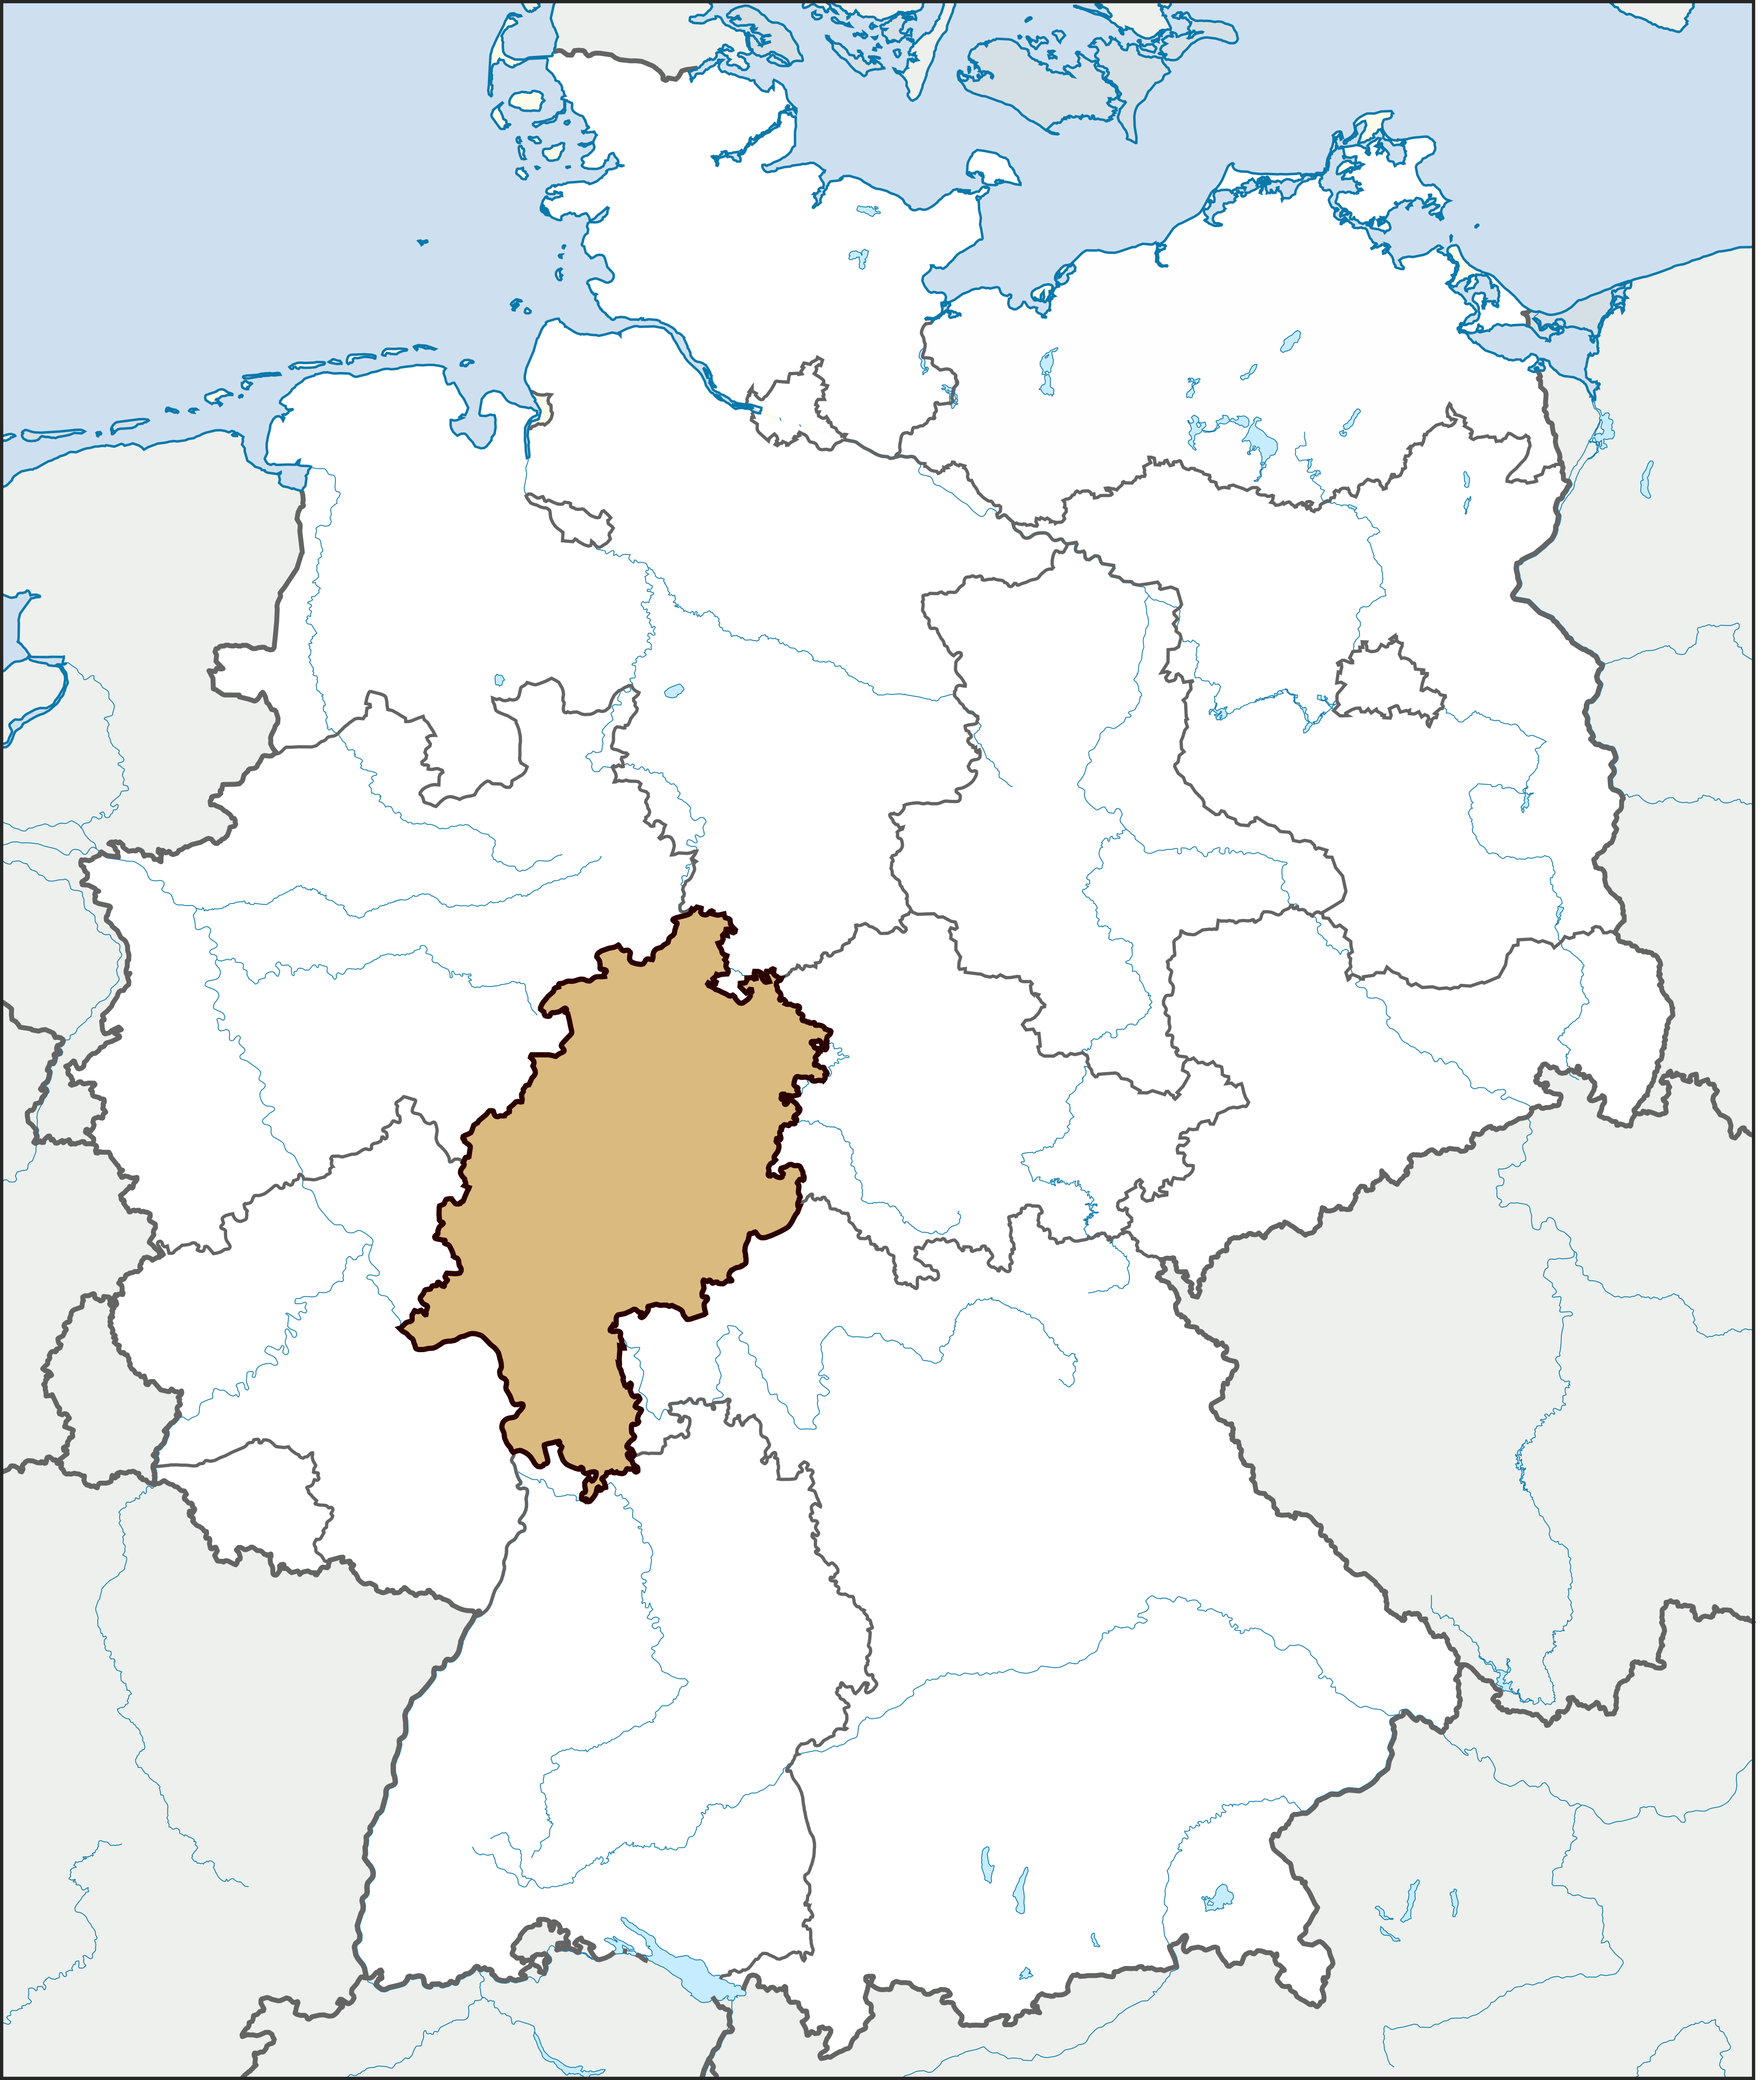
\includegraphics[width=0.45\textwidth]{Hesse_in_Germany.v1.0}
    \caption{Location of Hesse in the German Federal Republic}
\end{wrapfigure}

In order to represent the diversity of the population of \ac{iPD}-patients at \UKM and to ensure a balanced study cohort, as many of the treated patients as possible should be given the opportunity to participate in the \textsc{HessenKohorte}. Accordingly, the management of the study will adopt the recruitment strategies that have been successfully tested in previous clinical studies and to adapt them to the requirements of the long-term cohort study. To this end, on the one hand, patients are directly offered participation in the study during their appointments in the outpatient clinic of the hospital or during their inpatient stay in the Neurology Department. Secondly, members of \ac{PANAMA} will be made aware of the study with the aim of arousing the interest of potential participants. Finally, detailed information will be made available on the media website of \UKM to ensure sufficient information (\url{https://www.uni-marburg.de}).
\newpage

%%%%%%%%%%%%%%%%%%%%%%%%%%%%%%%%%%%%%%%%%%%%%%%%%%%%%%%%%%%%%%%%%%%%%%%
%%%% 										START OF SYNOPSIS												%%%%
%%%%%%%%%%%%%%%%%%%%%%%%%%%%%%%%%%%%%%%%%%%%%%%%%%%%%%%%%%%%%%%%%%%%%%%

\section{Protocol synopsis}
\inputtable{table_protocol_synopsis.tex}
\newpage

%%%%%%%%%%%%%%%%%%%%%%%%%%%%%%%%%%%%%%%%%%%%%%%%%%%%%%%%%%%%%%%%%%%%%%%
%%%% 										END OF SYNOPSIS													%%%%
%%%%%%%%%%%%%%%%%%%%%%%%%%%%%%%%%%%%%%%%%%%%%%%%%%%%%%%%%%%%%%%%%%%%%%%

\section{Study objectives and endpoints}
\subsection{Study objectives}
The primary aim of the \textsc{HessenKohorte} is to deepen the understanding of the development of \ac{QoL} in people with \ac{iPD} and to identify factors that have a beneficial or detrimental effect on it in a representative German cohort. In addition, the study aims to improve our understanding of the impact of the disease on caregivers and to find out which factors or forms of structural support make these carers more resilient to the stresses of caring for a person with \ac{iPD}.

\subsection{Primary study endpoint}
The primary endpoint of the \textsc{HessenKohorte} is the index patients' \ac{QoL}. A model has been developed to measure not only disease-related aspects of quality of life (\ac{CHAPO-PD}), but also additional factors that promote \ac{QoL} and thus go beyond health-related issues. This will be assessed using established questionnaires such as the \ac{PDQ39}\citep{jenkinson1997pdq39} or the \ac{WHOQoL}\citep{group1998world} and may be related to other characteristics of the patients included.

\subsection{Secondary study endpoint}
According to the large number of possible analyses and secondary endpoints for consideration, the authors foresee a substantial
number of analyses to be conducted in order to contemplate changes over time. Yet, a list of a few possible secondary endpoints shall be named:
\begin{itemize}[noitemsep,topsep=0pt]
  \item{Changes in motor symptoms of the index patient after up to 20 years}
  \item{Development of non-motor symptoms over up to 20 years}
  \item{Changes of the structural imaging over the observational period} 
\end{itemize}
Notwithstanding the unique characteristics of a study of the \ac{QoL} of people with \ac{iPD}, standard examinations of \ac{iPD} patients should also be carried out as far as the secondary endpoints are concerned. At this point, motor and non-motor symptoms should be mentioned as the most commonly encountered symptoms. The former are the hallmark of the disease, while the latter are increasingly recognised as responsible for huge losses in \ac{QoL} \citep{klietz2020qol}. The extent of motor symptoms is operationalised by Part III of the \ac{MDS-UPDRS}\cite{goetz2007updrs}. Non-motor symptoms will be measured using the \ac{NMSQ}, a measure capable of capturing a wide range of different aspects of this symptom domain. An overview of the scheduled time points for all questionnaires can be found in the table \ref{tab:questionnaireSchedule}.

\section{Study design}
The \textsc{HessenKohorte} is a longitudinal, observational, natural history study to assess the \ac{QoL} progression of study participants with \ac{iPD}. The planned cohort size of \num[round-precision = 0, round-mode = places]{1000}{} will be comprehensively assessed over a maximum of twenty years. All subjects and their relatives will undergo clinical examinations and patients will be regularly assessed for motor, non-motor, cognitive and neuropsychiatric symptoms and \ac{QoL}. Imaging studies will also be undertaken and patients will be asked to provide biospecimens including blood, urine, saliva, hair and faeces. All carers will be asked to complete questionnaires and provide digital data as part of the Hessen cohort.

\subsection{Scale and duration}
The study will accompany up to \num[round-precision = 0, round-mode = places]{1000}{} patients over at most 20 years to enable a profound insight into the life course of patients' and relatives' \ac{QoL}.

\subsection{Justification for study design}
The \textsc{HessenKohorte} is a single-centre, longitudinal, observational follow-up study of the \ac{QoL} of patients with \ac{iPD}. This unique primary endpoint will be assessed using a newly developed questionnaire, the main feature of which is a holistic assessment that looks not only at disease-related limitations but also at the existing resources and social environment of those affected by \cite{thieken2022jpd}. Accordingly, the involvement of family members is fundamental to understanding the impact of the disease on the patient's entire environment. The comparatively large number of subjects should provide a good insight into the lives of \ac{iPD} patients with their diverse phenotypes, but also offer opportunities for diverse investigations through the additional collection of biospecimens.

\subsection{Hypotheses}
\label{sec:hypoTheses}
The primary endpoint of the study is the development of \ac{iPD}-patients' \ac{QoL} over the course of up to 20 years. The \textsc{HessenKohorte} thereby addresses the following main scientific hypothesis:
\begin{itemize}
  \item Exploratory analysis of the development of \acl{QoL} over the course of the disease.
\end{itemize}
The design of the study is based on the currently accepted assumption that the \ac{QoL} of people with PD is significantly correlated with the severity of symptoms. It can also be assumed that the \ac{QoL} of people with PD is strongly related to that of their relatives. The present study design is intended to contribute to the longitudinal assessment of \ac{QoL}, but in particular to allow exploratory studies during or at the end of the data collection, which could provide information on whether certain factors in the behavioural data, imaging or biospecimens provided might have a predictive value for changes, but especially for reduced QoL.
% der letzte Satz klingt etwas hazy fuer mich. was ist da die Aussage?
% David: Stimmt. So besser verständlich?

\subsection{Planned analyses}
Our main method for assessing the hypotheses are \ac{ANOVA}, linear regression and correlation analyses. In particular we will analyse the correlation between the \ac{QoL} of the index patient and of her relatives and caregivers. In order to extend this analysis we will assess different influencing factors as e.g. age, gender and symptom burden (motor and non-motor). Furthermore in an attempt to elucidate the causal form of the interdependence we will analyse how \ac{QoL} of patients/caregivers at earlier timepoints relates to \ac{QoL} of caregivers/patients at a later point in time.

With regard to our hypothesis concerning the prediction of disease progress, we will primarily rely on linear and regression methods. We will try to offer models predicting disease symptoms at the end of the study compared to the status at earlier timepoints. While we first will look at a linear relationship we will also consider more complicated models when they are necessary to model disease progress convincingly. Also in this analysis mediating or moderating variables especially from sociodemographic data may play a role and will accordingly be considered.

\begin{figure}[h]
\label{fig2:scheme}
\centering
\includegraphics[width=1\textwidth]{Schema_HessenKohorte.v1.0}
\caption{Schematic overview of the planned analyses. Subjects will be enrolled subsequently and will receive regular follow-ups. In addition to clinical data in form of different questionnaires, biomarkers including cranial \ac{MRI}, blood, saliva, urine, hair and stool samples will be collected at an annual basis.}
\end{figure}


\section{Subject selection}
\label{sec:study_selection}
\subsection{Study population and Eligibility}
\label{sec:study_population}
Study candidates will be drawn from the patients treated in the Neurology Department of the \UKM, as either in- or outpatients. Moreover, all patients in the federal state of Hesse suffering from \ac{iPD} may submit a request for participation in the study. The inclusion and exclusion criteria (cf. Section \ref{sec:inclusion_criteriaIPS}) are checked by one of the study physicians, who are responsible for the final decision. Advertising for the study can be found in the form of a flyer, which is available in the Department of Neurology, but also in the form of an internet homepage, where the project will be presented to the public and we will promote study participation over the \ac{PANAMA} network.

\subsection{Inclusion and exclusion criteria \ac{iPD}-patients}
\label{sec:inclusion_criteriaIPS}
Subjects who meet all the following inclusion criteria may be given consideration for inclusion in this cohort study, provided no exclusion criteria are met (for both, cf. Table \ref{tab:inclusionexclusionCriteriaPatients}).

\inputtable{table_inclusion_and_exclusion_criteria_patients.tex}

\subsection{Inclusion criteria \ac{iPD}-patients' relatives}
\label{sec:inclusion_criteriaREL}
Only if a patient is included, the relatives may be asked for participation in the study. Subjects who agree to take part in the \textsc{HessenKohorte} must meet all the following inclusion and exclusion criteria (cf. Table  \ref{tab:inclusionexclusionCriteriaRelatives}).

\inputtable{table_inclusion_and_exclusion_criteria_relatives.tex}

\section{Subject accountability}
\subsection{Point of enrollment}
Subject will be considered to be enrolled at the time of the study-specific \ac{ICF} execution. No study-related procedures or assessments can take place until the \ac{ICF} is signed.

\subsection{Withdrawal}
All enrolled subjects (including those who have dropped out) must be recorded and documented. In case participants drop out of the study, an end-of-study form (\ref{sec:EOSform}) must be filled out and asked for the reasons for dropping out. 
% TODO this (reasons) has to be implemented in the form yet

Reasons for withdrawal include but are not limited to:
\begin{itemize}
  \item subject or relative choice to withdraw consent
  \item lost to follow-up
  \item pregnancy\footnote{\label{note1} only MR-imaging will be discontinued during pregnancy or from the moment of an implantation onwards.}
  \item implantation of electrical devices or metal parts in or on the body\footref{note1}
\end{itemize}

Subjects may withdraw at any time, with or without reason, and without prejudice to further treatment. The applicable \ac{CRF} up to the point of subject withdrawal and an end-of-study form \ref{chap:appendix} must be completed. A minimum of three documented attempts to contact any subject considered lost to follow-up should be made prior to completion of the end-of-study form. No further study data should be collected after the point at which a subject is withdrawn from the study or withdraws consent, for whatever reason. Data collected up to the time of subject withdrawal may be used. Subjects withdrawn after implantation will not be replaced.

% which 'implant procedure'?
%TODO: We need to draw and End-of-Study-Form @Steffi

\subsection{Lost to follow-up}
Patients who do not react to the invitation to fill ou the questionnaires will be contacted in total three times per mail or email:
\begin{itemize}
\item 30 days before the planned visit
\item at the date of the visit and
\item 30 days thereafter
\end{itemize}
If there is no response to the third contact attempt, patients are contacted by telephone to find out if there is a problem. Patients who cannot be contacted will receive the same number of mails/calls after one and two years. If there is no response for three years, an end of study form (see \ref{}) will be completed and the subject will be excluded. Vacancies due to excluded subjects may be filled 5 and 10 years after the start of the study.

% Urs: Ist das end-of-study form schon on im Appendix?

\subsection{Subject status and classification}
A subject will be considered enrolled in this study at the time of the study-specific \ac{ICF} execution.

\subsection{Enrolment control}
The overall enrollment in the study will be capped at \num[round-precision = 0, round-mode = places]{1000} participants.

\subsection{End-of-study definition}
The study is considered complete when 20 years from the first enrolment are over, in the year 2042.

\section{Study methods}
\subsection{Data collection}
The data collection schedule is shown in Table \ref{tab:DataCollectionPatients}
\inputtable{table_data_collection_schedule_patients.tex}
\inputtable{table_data_collection_schedule_relatives.tex}
%Urs: Bitte angleichen an das Protokoll zur Veröffentlichung


\subsection{Candidate screening}
\label{subsec:screening}
Subjects will be screened for participation in the study based on study inclusion and exclusion criteria as listed in Section \ref{sec:study_selection}. Subjects who have provided informed consent and who have been determined to not meet all eligibility requirements will not be considered.

\subsection{Informed consent}
Written informed consent must be obtained from potential study candidates and enrollment is only valid, after subjects sign and date the \ac{ICF}. The informed consent forms of this study can be found in appendices \label{sec:icf_patient} and \label{sec:icf_relative} respectively.
% @@urs

\begin{itemize}[noitemsep, topsep=0pt]
\item Subjects will be asked to sign the \ac{ICF} before study-specific tests or procedures are performed.
\item The idea of the study must be explained, and subjects must be given the time and opportunity to ask questions and have those questions answered to their satisfaction.
\item The \ac{ICF} is study specific and has been approved by the ethics commitee.
\item Written informed consent must be recorded appropriately by means of the subject’s dated signature.
\end{itemize}

\subsection{Questionnaires}
\label{subsec:questionnaires}
\subsubsection{\acl{CHAPO-PD}}
\label{questionnaires:chapo}
The backbone of the study will be the investigation of \ac{QoL}. Recent debates suggest that established measurement tools do not capture \ac{QoL} with a holistic view but focus on the health-related experience of \ac{QoL} [https://doi.org/10.3390/jpm12050804; https://doi.org/10.1007/s40273-016-0389-9]. Furthermore, it is unclear to date what determinants influence \ac{QoL} beyond mere disease in \ac{iPD}. It is also unclear how \ac{QoL} develops over the course of the disease. The HessenKohorte offers a unique opportunity to capture changes in \ac{QoL} in a large study population and develop a comprehensive understanding of this important concept. The study therefore pursues two goals: (i) the development and validation of a holistic measurement instrument for the assessment of \ac{QoL} and (ii) the longitudinal observation of \ac{HRQOL} using established measurement instruments (cf. Table 1). 
To fulfil the first goal, an instrument will be developed in the first year of the cohort in an evidence-based, patient-oriented and participatory manner, which will be validated alongside the cohort from the second year onwards.  This means that in addition to a systematic review of existing studies, \ac{iPD} patients will be interviewed about their personal experience of \ac{QoL} and actively involved in the development process of the instrument according to the INVOLVE-guideline \url{https://www.invo.org.uk/wp-content/uploads/2019/04/Copro_Guidance_Feb19.pdf}. In this process, the study team is guided by the work from the NRW80+ study in which the experience of \ac{QoL} of elderly people was investigated for the first time in Germany \url{https://doi.org/10.1007/s00391-017-1217-3}.
% Urs: Diesen Teil soll Marlena schreiben.

\subsubsection{\acl{MDS-UPDRS} (\acs{MDS-UPDRS})}
%Urs: Sollen wir das nicht auch in das Protokoll packen? Meine Idee wäre, dass man das einfach ausdrucken kann und alles zusammen hat für ein Visit.
\label{questionnaires:updrs}
The \ac{MDS-UPDRS} \cite{goetz2007updrs} evaluates various aspects of \ac{iPD}-patients, including non-motor and motor symptoms. It consists of four parts:
\begin{itemize}
\item Part I: Experiences of daily living (non-motor symptoms), including 13 items.
\begin{itemize}
\item A: Behavioral problems of the patient, as evaluated by the examiner.
\item B: Part on non-motor symptoms completed by the patient, with the assistance of a caregiver if necessary, but independent of the investigator.
\end{itemize}
\item Part II: Experiences of daily living (motor aspects) with 13 items. This part is also a self-report questionnaire to be completed by the patient, with the assistance of a caregiver if necessary, but independent of the investigator.
\item Part III: Motor examination with 18 items. All instructions are read to the patient by the examiner or demonstrated directly, so that this part is completed by the examiner.
\item Part IV: Motor Complications with 6 items. This part contains instructions for the examiner and also instructions to be read to the patient. It combines patient-related information with clinical observations and assessments by the examiner.
\end{itemize}

\subsubsection{\acl{MoCa} (\acs{MoCa})}
\label{questionnaires:MoCa}
The \acl{MoCa} evaluates the performance in different cognitive domains. The questions test cognitive abilities such as memory, language production , contextual thinking, attention and concentration, behavior, arithmetic, temporal and spatial orientation, and the ability to recognize complex shapes and patterns. Scores result from the correct completion of the tasks, whereby the cognitive performance in the individual domains but also as an overall score can be quantified. The \ac{MoCa} was developed in 2005 \cite{nasreddine2005moca} and has been used in clinical practice since then. The test must be administered by an examiner, who is separately trained and an assessment sheet, a pen and stopwatch are needed. The duration is about \num[round-precision = 0, round-mode=places]{10} \SI{}{\minute}.

\underline{Psychometrics:}
\inputtable{table_psychometrics_moca.tex}

\subsubsection{\acl{NMSQ}, (\acs{NMSQ})}
\label{questionnaires:NMSQ}
The \ac{NMSQ} is a 30-item rater-based scale designed to assess a broad spectrum of non-motor symptoms in patients with \ac{iPD}.
The \ac{NMSQ} measures the severity and frequency of non-motor symptoms across nine dimensions (??).
%TODO: More information is needed on what the domains are and what to consider, etc.

\subsubsection{\acl{BDI} (\acs{BDI})}
\label{questionnaires:BDI}

The \acl{BDI} measures the severity of depressive symptoms. It consists of 21 items  measuring symptoms on a scale from 0--3. The questionnaire was first introduced in 1991 \cite{beck1987bdi1} and revised to the current version in 1996 \cite{beck1996bdi2}. The self-administered test takes \numrange{5}{10} \SI{}{\minute} to be completed but does not require any special training. Answers are added for the total score, so that results range in a scale of 0--63 points. Higher scores thereby correspond to more severe symptoms. Since its development, the \ac{BDI} has been used to quantify depressive symptoms in non-specific populations, but particularly in patients with stroke, spinal cord injury and \ac{iPD}. 

\underline{Scores:}
\begin{itemize}\itemsep2pt
\item 0--12: no depressive symptoms or clinically inapparent
\item 13--19: mild depressive syndrome
\item 20--28: moderate depressive syndrome
\item $>$ 29 severe depressive syndrome
\end{itemize}

\underline{Psychometrics:}
\inputtable{table_psychometrics_bdi.tex}

\subsubsection{\acl{CBI} (\acs{CBI})}
\label{questionnaires:CBI}
The \acl{CBI} assesses the presence or severity of symptoms indicative of burnout. In the short version used, the questionnaire consists of 19 items that scale levels of physical and psychological exhaustion in relation to personal, work and client burnout. The CBI was introduced in 2005 by Kristensen et al. \cite{kristensen2005cbi} and is self-administered without special training. It takes about 5-10 minutes to complete. The scale ranges from 1 (``never/very seldom'' or ``to a very low degree'') to 5 (``very often'' or ``to a very high degree''), resulting in a total score of 19--95 by adding the individual scores or individual scales for personal burnout (6--30), work-related burnout (7---36) and client-related burnout (6--30). A higher score indicates higher levels of stress and an increased likelihood of burnout.

\underline{Psychometrics:}
\inputtable{table_psychometrics_cbi.tex}

\subsubsection{\acl{CISS} (\acs{CISS})}
\label{questionnaires:CISS}
The \acl{CISS} assesses habitual coping with stress in the context of task-oriented coping, emotion-oriented coping and avoidance-oriented coping with a total of 24 and 48 questions respectively. The CISS was originally introduced in 1990 \cite{endler1990ciss} and revised in 2020 for a shortened, German-language version \cite{kalin2020ciss}. The questionnaire is self-administered without special training and takes 10--15 minutes to complete.

%TODO: add further details to how the score is determined, @David?

\underline{Psychometrics:}
\inputtable{table_psychometrics_ciss.tex}

\subsubsection{\acl{MFI-20}}
\label{questionnaires:MFI20}
The \acl{MFI-20} measures 5 dimensions of fatigue with 20 questions: general fatigue, physical fatigue, reduced activity, reduced motivation and mental fatigue. The \acs{MFI-20} was introduced in 1995 \cite{smets1995mfi20}. It is a self-administered test that requires no special training and is reported to take 5--10 minutes to complete. It includes response options to various fatigue-related statements ranging from ``Yes, this is true'' to ``No, this is not true'', scaled from 1 -- 5 per question, with 4 -- 20 points for each dimension. A high total score on the different dimensions corresponds to a higher level of fatigue in the corresponding dimension.

\underline{Psychometrics:}
\inputtable{table_psychometrics_mfi20.tex}

\subsubsection{\acl{PDCB} (\acs{PDCB})}
\label{questionnaires:PDCB}
The `Parkinson's Disease Caregiver Burden Questionnaire''  (\acs{PDCB}) measures level of burden experienced in caring for a person with \ac{iPD}. It consists of 20 questions in 8 domains that indicate the occurrence of various emotional, health and social consequences of caring for persons with \ac{PD}, using a 0--4 point scale by disagreeing (``I disagree'') and gradually increasing agreement (``I strongly agree'') with statements about one's burden. The (\acs{PDCB}) was first introduced in 2013 \cite{zhong2013pdcb}, and revised in 2019 with a German translation \cite{klietz2019pdcb}. It takes 5 -- 10 minutes to be completed and is a self-administered test that requires no special training. The total score of the questionnaire is obtained by adding the individual scores between 0 -- 4 of all 20 questions. A higher score corresponds to a greater burden of caring for a person with \ac{PD}.

\underline{Psychometrics:}
\inputtable{table_psychometrics_pdcb.tex}

\subsubsection{\acl{PHQ}}
\label{questionnaires:PHQ}
The ``Patient Health Questionnaire'' (\acs{PHQ}) is an instrument for the diagnosis of mental disorders that assesses various somatic, psychological and stress-related complaints on the basis of 16 domains. The \acs{PHQ}, which is based on DSM-IV criteria, was introduced for psychodiagnosis in the USA in 1999 \cite{spitzer1999phq} and validated in 2002 as the ``Health Questionnaire for Patients (PHQ-D)'' in a German version \cite{lowe2002phq}. It takes about 15 minutes to complete and is self-administered. Nine of the items (2a--2i) measure ``depressiveness''. The response categories are as follows: 0 (``not at all''), 1 (``on some days''), 2 (``on more than half of the days'') and 3 (``almost every day''), giving a score of 0--27. Scores below 5 points indicate no depressive symptoms, 5--10 points indicate mild depressive symptoms and all scores above 10 points indicate major depression (moderate, marked or severe). A further 15 items (1a--1m, 2c, 2d) measure somatic symptoms, resulting in a scale total for the `somatic symptoms''. Of these, 13 items are scored as: 0 (``not impaired''), 1 (``slightly impaired'') or 2 (`severely impaired''). In addition, two items from the depression section are scored as: 0 (``not at all''), 1 (``on some days''), 2 (``on more than half of the days'') and 3 (``almost every day''). The total score ranges from 0--30 points, with higher scores corresponding to greater somatoform distress. 
A severity score for the stress domain can be obtained by summing items 12a--12j to obtain a` scale total. The numerical rating of the individual items is 0 ('not affected'), 1 ('slightly affected') or 2 ('severely affected'). Accordingly, the total stress score varies between 0 and 20, with higher scores corresponding to greater stress.

\underline{Psychometrics:}
\inputtable{table_psychometrics_phq.tex} %TODO: The values are missing, as well as the source,@David?

\subsubsection{\acl{PSS} (\acs{PSS})}
\label{questionnaires:PSS}
Der „Perceived Stress Scale“ ist eine Selbstauskunft, die das Ausmaß bewertet, in dem der Befragte Situationen in seinem Leben im letzten Monat als stressig empfunden hat und erfasst dabei sowohl eine Skala der Hilflosigkeit als auch der Selbstwirksamkeit. Der PSS-Fragebogen besteht aus 10 Fragen, die das Stressempfinden im letzten Monat in Ihrer Häufigkeit auf einer Skala von „Nie“ bis „Fast immer“ erfassen. Erstmalig wurde der PSS 1983 eingeführt (Cohen et al. 1983) und 2010 in eine deutsche Verfassung überarbeitet (Schneider et al. 2010). 
Die Durchführung dauert etwa 5 Minuten und erfordert kein gesondertes Training. Die Antwortmöglichkeiten auf der Skala von „Nie“ bis „Fast immer“ entsprechen einer Punkteskala von 1-5. Die Skala der Hilflosigkeit ergibt sich aus der Summe der Items 1, 2, 3, 6, 9, 10; die Skala der Selbstwirksamkeit aus der Summe der Items 4, 5, 7, 8. Für die Berechnung des Gesamtscores müssen die Items 4, 5, 7 und 8 der Selbstwirksamkeitsskala invertiert werden. Der Gesamtscore berechnet sich aus der Summe der Items der Hilflosigkeitsskala und der Summer der invertierten Items der Selbswirksamkeitsskala. Höhere Werte deuten auf ein erhöhtes Stresslevel hin.

\underline{Psychometrics:}
\inputtable{table_psychometrics_pss.tex}

\subsubsection{\acl{WHOQoL} (\acs{WHOQoL})}
\label{questionnaires:WHOQoL}

Der Fragebogen “World Health Organization Quality of Life – BREF” erfasst die subjektive Lebensqualität im Erwachsenenalter und besteht aus insgesamt 26 Items, die den 4 Domänen Physische Lebensqualität, Psychische Lebensqualität, Soziale Beziehungen und Umwelt zugeordnet sind. Dazu wird anhand von 2 zusätzlichen Items die globale Lebensqualität und generelle Gesundheit abgefragt. Im Auftrag der World Health Organisation wurde der Fragebogen 1996 eingeführt und in deutscher Übersetzung seit 2016 angewendet.

Die Bearbeitungsdauer wird mit 10 – 15 Minuten angegeben. Anhand der Antwortmöglichkeiten werden die Domänen durch eine Punkteskala (1-5) wie folgt quantifiziert, wobei eine höhere Punktzahl einer besseren Lebensqualität entspricht:

\underline{Scores:}
\begin{itemize}\itemsep2pt
\item Physical health: 7 -- 35 points
\item Psychological Health 6 -- 30 points
\item Social relationships 3 -- 15 points %TODO:  Is that the correct translation? @David?
\item Environment 8 – 40 points
\end{itemize}

\underline{Psychometrics:}
\inputtable{table_psychometrics_whoqol.tex}

\subsection{Biosamples}
\label{subsec:biosamples}

\subsubsection{Blood}
\label{biosamples:blood}


\subsubsection{Urine}
\label{biosamples:urine}

\subsubsection{Saliva}
\label{biosamples:saliva}
Es erfolgen zwei Sammkungen von Speichelproben mit unterschiedlichem Ziel. Zum einen soll eine Analyse der Metabolomics bei den \ac{iPS}-Patienten erfolgen, zum anderen eine DNA-Extraktion. Es sind keine Vorbereitungen für die Probenentnahme notwendig.

Für die Anylse der Metabolomics erfolgt die Sammlung des Speichels mittels Salivette (Sarstedt??). Hierzu erfolgt die Entnahme nach ``unstimulated whole-mouth wash'' und es werden zwei Röhrchen gefüllt. Daneben wird eine Probe mittels Kaugummi erfolgen, die zusammen mit dem Kaugummi zentrifugiert wird bevor das Kaugummi entsorgt wird.  Die anschließend homogenisierte Probe wird in Aliquots von  \SI{150}{\micro\litre} gefüllt und bei -80°C gelagert.

Die DNA-Extraktion aus Speichelproben erfolgt mit dem SalivaGene Collection Module II System. Dieses System vereinfacht die Entnahme und Lagerung der Proben durch einfache Handhabung. Die Proben werden bis zu 12 Monate bei -80°C gelagert und anschließend im CMBBR prozessiert. 

Benötigte Materialien
\begin{itemize}
\item Invitek SalivaGene Collection Module II (Artikelnummer: 10 352 122 00)
\item Sarstedt Salivette (Artikelnummer: 51.1534.500)

\end{itemize}

\subsubsection{Hair}
\label{biosamples:hair}
Metabolomics is a useful tool for identifying biomarkers of disease and uncovering pathogenic mechanisms [10.3389/fchem.2021.674265]. However, most metabolomic studies use biological fluids such as blood and urine as biospecimens, which can be dramatically affected by daily activities and dietary variations, resulting in measurement variability. In contrast, hair can serve as a robust source of stable longitudinal metabolite information. Human hair grows at a rate of approximately \num{1} \SI{}{\centi\metre} per month, with both endogenous compounds and environmental factors being incorporated into the hair during growth. Therefore, we plan to analyse hair metabolomics over time during the course of the study. For this purpose, an in-house questionnaire on hair characteristics and products used has been developed and will be administered to all patients. A specific protocol has been developed for hair collection, including standardised location of hair to be collected, technique and processing. 

Hair samples are taken from the posterior vertex using a standardised procedure. Along with a questionnaire asking about the use of specific products, 2-3 strands of hair are cut as close to the skin as possible. The collected hairs are wrapped in foil and stored in a dark place until processing. Further details of the procedure are given in the appendix (see chapter \ref{chap:appendix}).

\subsubsection{Stool}
\label{biosamples:stool}


\subsection{\ac{MRI}}
\label{subsec:MRI}
Every enrolled patient will receive an \ac{MRI} if there is no contraindication and if the patient wishes. To maximise synergy with other large studies at the centre and to ensure high quality sequences, the programme to be undertaken has been based on the PPMI study\footnote{\url{https://www.ppmi-info.org/}}. Further details are provided below.
\subsubsection{Overview of MR-imaging}
\inputtable{table_mri_overview.tex}

\subsubsection{Procedure of the imaging}
Participants should be positioned comfortably and correctly to minimise movement during the scan. Technicians are also instructed to observe the following
\begin{itemize}[noitemsep,topsep=0pt]
\item Subjects should be informed of the total acquisition time and positioned for maximum comfort.
\item The subject's head should be positioned comfortably and supine in the head coil to minimise any movement during the scan.
\item Proper back support and support under the knees should provide greater comfort and result in less movement during the scan.
\item There should be no left-right or ear-to-shoulder head tilt and the subject's neck should not be extended or retracted.
\item The subject's head should be centred in the head coil using the nasion as an anatomical landmark. It is recommended that the subject is positioned high enough in the coil to avoid signal loss in the lower parts of the brain.
\item Immobilisation devices such as Velcro straps or foam padding should be used to reduce movement.
\item The positioning lasers should be used to align the nasion with the isocentre of the magnets.
\end{itemize}
If the length of a subject's neck does not allow proper positioning in the head coil, please document this on the \ac{MRI} acquisition document along with any other pertinent information regarding the subject's scan session.

\newcolumntype{s}{>{\hsize=.3\hsize}X}
\subsubsection{T1-weighted, 3D volumetric sequence}
\inputtable{table_mri_t1_3d.tex}

\subsubsection{2D Gradient-echo T2*-weighted EPI}
\inputtable{table_mri_2d_gradient_echo.tex}


\subsubsection{2D Gradient recalled echo with MT preparation}
\inputtable{table_mri_2d_gradient_recalled_echo_with_MT_preparation.tex}

\subsubsection{REPEAT T2-weighted}
\inputtable{table_mri_2d_repeat_t2_weighted.tex}

\subsubsection{2D Diffusion-weighted EPI}
\inputtable{table_mri_2d_diffusion.tex}

\subsubsection{3D T2 \ac{FLAIR} Sequence}
\inputtable{table_mri_3d_t2_FLAIR.tex}

\section{Visits}
Table \ref{tab:questionnaireSchedule} provides a tabular presentation of the visits and the parameters and values collected. Below is a detailed description of each scheduled appointment.

\inputtable{table_questionnaire_schedule.tex}

\subsection{Baseline visit \ac{iPD}-patients}
All potential candidates will undergo screening procedures (see Section \ref{subsec:screening}). Subjects are not required to be on stable antiparkinsonian medication prior to informed consent, nor are they required to be receiving regular treatment at the \UKM. Subjects meeting all inclusion criteria and none of the exclusion criteria (see Table \ref{tab:inclusionexclusionCriteriaPatients}) may be enrolled. The baseline visit can take place at any time after screening and is the final determination of eligibility for the study. The following data and samples should be collected from patients at the baseline visit:
\begin{itemize}[noitemsep,topsep=0pt]
\item General Assessments
\begin{itemize}[noitemsep,topsep=0pt]
\item Demographic data and personal information
\item Medication schedule
\end{itemize}
\item Questionnaires
\begin{itemize}[noitemsep,topsep=0pt]
\item \acl{CHAPO-PD} -- \acs{CHAPO-PD} (cf. Section \ref{subsec:questionnaires}\ref{questionnaires:chapo})
\item \acl{MDS-UPDRS} -- \acs{MDS-UPDRS} (cf. Section \ref{subsec:questionnaires}\ref{questionnaires:updrs})
\item \acl{MoCa} -- \acs{MoCa} (cf. Section \ref{subsec:questionnaires}\ref{questionnaires:MoCa})
\item \acl{NMSQ} -- \acs{NMSQ} (cf. Section \ref{subsec:questionnaires}\ref{questionnaires:NMSQ})
\item \acl{PDQ39} -- \acs{PDQ39} (cf. Section \ref{subsec:questionnaires}\ref{questionnaires:PDQ39})
% PDQ-39 scheint nicht dabei zu sein bisher. Bitte einmal mit MArlena besprechen, ob wir den brauchen oder nicht.
\item \acl{BDI} -- \acs{BDI} (cf. Section \ref{subsec:questionnaires}\ref{questionnaires:BDI})
\item \acl{MFI-20} -- \acs{MFI-20} (cf. Section \ref{subsec:questionnaires}\ref{questionnaires:MFI20})
\item \acl{PHQ} -- \acs{PHQ} (cf. Section \ref{subsec:questionnaires}\ref{questionnaires:PHQ})
\item \acl{PSS} -- \acs{PSS} (cf. Section \ref{subsec:questionnaires}\ref{questionnaires:PSS})
\item \acl{WHOQoL} -- \acs{WHOQoL} (cf. Section \ref{subsec:questionnaires}\ref{questionnaires:WHOQoL})
\end{itemize}
\item Biosamples
\begin{itemize}[noitemsep,topsep=0pt]
\item Blood sample (cf. Section \ref{subsec:biosamples}\ref{biosamples:blood})
\item Urine sample (cf. Section \ref{subsec:biosamples}\ref{biosamples:urine})
\item Saliva sample (cf. Section \ref{subsec:biosamples}\ref{biosamples:saliva})
\item Hair sample (cf. Section \ref{subsec:biosamples}\ref{biosamples:hair})
\item Stool sample (cf. Section \ref{subsec:biosamples}\ref{biosamples:stool})
\item \acl{MRI} -- \acs{MRI} (cf. Section \ref{subsec:MRI}) 
\end{itemize}
\end{itemize}

\subsection{Half year visit \ac{iPD}-patients ($\pm$ 100 days)}
In between the annual visits, there will be six-monthly visits that don't require patients to attend a study centre in person. There will be no neurological examination or biospecimen collection. Instead, we will collect questionnaire data, in particular on quality of life, symptoms of psychological distress and specific symptoms related to \ac{iPD}. These data will be collected either electronically or through paper questionnaires sent to patients. The following data should be collected from patients at the six-monthly visits:

\begin{itemize}[noitemsep,topsep=0pt]
\item General Assessments
\begin{itemize}[noitemsep,topsep=0pt]
\item Demographic data and personal information (if changed)
\item Medication schedule
\end{itemize}
\item Questionnaires
\begin{itemize}[noitemsep,topsep=0pt]
\item \acl{CHAPO-PD} -- \acs{CHAPO-PD} (cf. Section \ref{subsec:questionnaires}\ref{questionnaires:chapo})
\item \acl{NMSQ} -- \acs{NMSQ} (cf. Section \ref{subsec:questionnaires}\ref{questionnaires:NMSQ})
\item \acl{PDQ39} -- \acs{PDQ39} (cf. Section \ref{subsec:questionnaires}\ref{questionnaires:PDQ39})
% PDQ39 erscheint nicht in der Liste bisher. Marlena fragen
\item \acl{BDI} -- \acs{BDI} (cf. Section \ref{subsec:questionnaires}\ref{questionnaires:BDI})
\item \acl{MFI-20} -- \acs{MFI-20} (cf. Section \ref{subsec:questionnaires}\ref{questionnaires:MFI20})
\item \acl{PHQ} -- \acs{PHQ} (cf. Section \ref{subsec:questionnaires}\ref{questionnaires:PHQ})
\item \acl{PSS} -- \acs{PSS} (cf. Section \ref{subsec:questionnaires}\ref{questionnaires:PSS})
\end{itemize}
\end{itemize}

\subsection{Annual visit \ac{iPD}-patients ($\pm$ 100 days)}
Patients will be seen in person at the study centre (\UKM) once a year. During this visit we will collect biospecimens, questionnaire data and perform a functional neurological assessment. We will also assess whether the patient still meets the requirements for informed consent. If not, consent will be obtained from the patient's legal representative for continued participation in the study. The following data and samples will be collected from patients at the annual visit:

\begin{itemize}[noitemsep,topsep=0pt]
\item General Assessments
\begin{itemize}[noitemsep,topsep=0pt]
\item Demographic data and personal information
\item Medication schedule
\item Ability to consent with proceeding in the study
\end{itemize}
\item Questionnaires
\begin{itemize}[noitemsep,topsep=0pt]
\item \acl{CHAPO-PD} -- \acs{CHAPO-PD} (cf. Section \ref{subsec:questionnaires}\ref{questionnaires:chapo})
\item \acl{MDS-UPDRS} -- \acs{MDS-UPDRS} (cf. Section \ref{subsec:questionnaires}\ref{questionnaires:updrs})
\item \acl{MoCa} -- \acs{MoCa} (cf. Section \ref{subsec:questionnaires}\ref{questionnaires:MoCa})
\item \acl{NMSQ} -- \acs{NMSQ} (cf. Section \ref{subsec:questionnaires}\ref{questionnaires:NMSQ})
\item \acl{PDQ39} -- \acs{PDQ39} (cf. Section \ref{subsec:questionnaires}\ref{questionnaires:PDQ39})
% PDQ-39 scheint nicht dabei zu sein bisher. Bitte einmal mit MArlena besprechen, ob wir den brauchen oder nicht.
\item \acl{BDI} -- \acs{BDI} (cf. Section \ref{subsec:questionnaires}\ref{questionnaires:BDI})
\item \acl{MFI-20} -- \acs{MFI-20} (cf. Section \ref{subsec:questionnaires}\ref{questionnaires:MFI20})
\item \acl{PHQ} -- \acs{PHQ} (cf. Section \ref{subsec:questionnaires}\ref{questionnaires:PHQ})
\item \acl{PSS} -- \acs{PSS} (cf. Section \ref{subsec:questionnaires}\ref{questionnaires:PSS})
\item \acl{WHOQoL} -- \acs{WHOQoL} (cf. Section \ref{subsec:questionnaires}\ref{questionnaires:WHOQoL})
\end{itemize}
\item Biosamples
\begin{itemize}[noitemsep,topsep=0pt]
\item Blood sample (cf. Section \ref{subsec:biosamples}\ref{biosamples:blood})
\item Urine sample (cf. Section \ref{subsec:biosamples}\ref{biosamples:urine})
\item Saliva sample (cf. Section \ref{subsec:biosamples}\ref{biosamples:saliva})
\item Hair sample (cf. Section \ref{subsec:biosamples}\ref{biosamples:hair})
\item Stool sample (cf. Section \ref{subsec:biosamples}\ref{biosamples:stool})
\end{itemize}
\item \acl{MRI} -- \acs{MRI} (cf. Section \ref{subsec:MRI}) 
\end{itemize}

\subsection{Unscheduled visit \ac{iPD}-patients}
As a significant proportion of patients will be recruited from our outpatient clinic, it is expected that some patients will attend for reasons other than participation in the study, such as worsening symptoms and adjustment of their medication or \ac{DBS} device. If data relevant to the study are collected during these unscheduled visits (e.g. \ac{MDS-UPDRS} scores), these may be included in the study.
 
\subsection{Baseline visit relatives}
As this study is intended to enrol both patients and their relatives, there will also be a baseline visit for the patients' relatives. Relatives who meet all the inclusion criteria and none of the exclusion criteria (see Section \ref{sec:study_selection}) will then be enrolled. The baseline visit can take place at any time during the screening period and is the final determination of eligibility for the study. For the relatives, the following data will be collected through questionnaires:

\begin{itemize}[noitemsep,topsep=0pt]
\item General Assessments
\begin{itemize}[noitemsep,topsep=0pt]
\item Demographic data and personal information
\end{itemize}
\item \acl{BDI} -- \acs{BDI} (cf. Section \ref{subsec:questionnaires}\ref{questionnaires:BDI})
\item \acl{CBI} -- \acs{CBI} (cf. Section \ref{subsec:questionnaires}\ref{questionnaires:CBI})
\item \acl{CISS} -- \acs{CISS} (cf. Section \ref{subsec:questionnaires}\ref{questionnaires:CISS})
\item \acl{MFI-20} -- \acs{MFI-20} (cf. Section \ref{subsec:questionnaires}\ref{questionnaires:MFI20})
\item \acl{PDCB} -- \acs{PDCB} (cf. Section \ref{subsec:questionnaires}\ref{questionnaires:PDCB})
\item \acl{PSS} -- \acs{PSS} (cf. Section \ref{subsec:questionnaires}\ref{questionnaires:PSS})
\item \acl{WHOQoL} -- \acs{WHOQoL} (cf. Section \ref{subsec:questionnaires}\ref{questionnaires:WHOQoL})
\end{itemize}

\subsection{Half year visit relatives ($\pm$ 100 days)}
Similar to the procedure for patients, the half-yearly visit of relatives will mainly consist of a psychometric assessment, which will be carried out either electronically or by sending them questionnaires in paper form. The following measures will be collected:

\begin{itemize}[noitemsep,topsep=0pt]
\item General Assessments
\begin{itemize}[noitemsep,topsep=0pt]
\item Demographic data and personal information (if changed)
\end{itemize}
\item \acl{BDI} -- \acs{BDI} (cf. Section \ref{subsec:questionnaires}\ref{questionnaires:BDI})
\item \acl{CBI} -- \acs{CBI} (cf. Section \ref{subsec:questionnaires}\ref{questionnaires:CBI})
\item \acl{PDCB} -- \acs{PDCB} (cf. Section \ref{subsec:questionnaires}\ref{questionnaires:PDCB})
\item \acl{MFI-20} -- \acs{MFI-20} (cf. Section \ref{subsec:questionnaires}\ref{questionnaires:MFI20})
\item \acl{PSS} -- \acs{PSS} (cf. Section \ref{subsec:questionnaires}\ref{questionnaires:PSS})
\end{itemize}


\subsection{Annual visit relatives ($\pm$ 100 days)}
On an annual basis, the relatives are subjected to an extended data assessment, which can also take place at a distance, i.e. electronically or by post. The following information is collected from relatives during the annual visit:

\begin{itemize}[noitemsep,topsep=0pt]
\item General Assessments
\begin{itemize}[noitemsep,topsep=0pt]
\item Demographic data and personal information (if changed)
\end{itemize}
\item \acl{BDI} -- \acs{BDI} (cf. Section \ref{subsec:questionnaires}\ref{questionnaires:BDI})
\item \acl{CBI} -- \acs{CBI} (cf. Section \ref{subsec:questionnaires}\ref{questionnaires:CBI})
\item \acl{PDCB} -- \acs{PDCB} (cf. Section \ref{subsec:questionnaires}\ref{questionnaires:PDCB})
\item \acl{MFI-20} -- \acs{MFI-20} (cf. Section \ref{subsec:questionnaires}\ref{questionnaires:MFI20})
\item \acl{PSS} -- \acs{PSS} (cf. Section \ref{subsec:questionnaires}\ref{questionnaires:PSS})
\item \acl{WHOQoL} -- \acs{WHOQoL} (cf. Section \ref{subsec:questionnaires}\ref{questionnaires:WHOQoL})
\end{itemize}

\section{Data management}
% Bitte Urs idealerweise nichts daran ändern, sondern die THM dazu bekommen, dass sie die Treuhandstelle einrichten und wir das wie geplant machen können
% UK: das ist ein alter KOmmentar, oder? Wir machen es jetzt ohne THM(?)
% Ja, ohne THM. Nur ein Datenschutzkonzept brauchen wir wahrscheinlich trotzdem, oder? Habe auch noch einmal Gunter geschrieben (20.02.), um herauszufinden, wie das in der Epileptologie gehandhabt wird.

\section{Amendments}
For protocol amendments that may affect the rights, safety, or welfare of trial subjects or the scientific integrity of the data, a protocol amendment must be prepared. Appropriate approvals (especially from the ethics committee) of the revised protocol must be obtained prior to implementation.

\section{Compliance}
\subsection{Statement of Compliance}
This trial will be conducted in accordance with ICH-GCP and the ethical principles of the Declaration of Helsinki.

\subsection{Investigator responsibilities}

\subsubsection{Delegation of responsibilities}
If specific tasks are delegated, the investigator is responsible for providing appropriate training, if necessary, and adequate supervision of those to whom tasks are delegated. The investigator is responsible for regulatory violations resulting from failure to adequately supervise the conduct of the clinical trial.

\subsection{Ethics committee}
The trial site has received approval for the clinical trial from the local ethics committee. A copy of the written protocol approval is included in the appendix (see Chapter \ref{chap:appendix}). Any changes to the protocol must be reviewed and approved before the protocol is implemented. In addition, any changes to the \ac{ICF} must also be approved. If the study is extended to other centres, ethical approval must be obtained from the relevant ethics committee.
% Urs:  Ich bin sicher, ich habe das eingefügt aber brauchen wir das Ethikvotum hier?
% UK: ich denke eigentlich nicht

\section{Monitoring}
The majority of the interventions and examinations during the trial are observational, i.e. no interventions take place. Therefore, neither adverse events \ac{AE} nor serious adverse events \ac{SAE} are anticipated (cf. Section \ref{subsec:anticipated_AE}). However, all imaging sequences will be reviewed for pathological findings and participants will be followed up for incidental findings so that further action can be taken. In addition, if an adverse event occurs during blood collection, the study coordinator will be notified within 24 hours so that further action can be taken if necessary. Information about the risks of the study is provided in the following section (cf. Section \ref{subsec:anticipatedAE}).

\section{Potential Risks and Benefits}
\subsection{Anticipated Adverse Events}
\label{subsec:anticipated_AE}
Due to the nature of the \textsc{HessenKohorte} as observational study, most medial events and emergencies are not deemed \acl{AE}. Falls, infections and even death occur naturally in the course of \ac{iPD}, so that this study only aims at documenting these events to learn more about the natural course of the disease. \ac{AE} in the sense of this study are only those events which wouldn't have happened without study participations. These are exclusively complications arising from the sampling of data.

\subsection{Risks associated with the study participation}
There are no specific medical risks associated with participation in the Hessen cohort, as all participants have access to the standard of care for their condition. Risks associated with participation in the study therefore only arise from the collection of data, which is discussed below.

\subsection{Risks associated with the sampling of biodata}
While the collection of stool, hair, urine and saliva does not carry any particular risks, the collection of blood carries the usual, rather small, risks of numbness due to nerve damage or infection at the site of the venipuncture. Participants will be informed of these risks and measures will be taken to minimise them: blood collection will only be carried out by experienced personnel, preferably in the supine position. In the event of an \ac{AE}, this will be documented and a physician familiar with the study will be notified to take further action if necessary.
%Urs: haben wir das AE-Form schon drin?

\subsection{Risks associated with the \ac{MRI}}
\ac{MRI} is a radiological procedure that avoids X-rays and is generally well tolerated. The main risk comes from participants bringing metal objects into the \ac{MRI} scanner, which is dangerous because of the strong magnetic field inside. These objects can be either medical or aesthetic implants, remnants of previous accidents or war experiences, or they can be carried inadvertently, for example in a pocket, before entering the \ac{MRI} scanner. In this study, each participant will be thoroughly informed of this risk before each \ac{MRI} scan. Other potential problems will also be addressed, such as the loud noise and confined space inside the \ac{MRI} scanner. For the former, participants will be given medical grade ear protection to prevent hearing loss by reducing sounds to harmless intensities. With regard to psychological problems caused by the confined space, subjects will be screened for signs of claustrophobia before the scan. During the \ac{MRI}, participants can stop the scans at any time using a panic button given to them as soon as they enter the machine

\section{Informed consent}
Participants cannot be enrolled in the study until they have been adequately informed and have signed the \ac{ICF}. The relevant documentation can be found in the appendix to this document. (see chapter \ref{chap:appendix}).

\section{Termination of the study}
The study will be terminated when the last subject has had her/his last visit in the year 2042 and the end-of-visit-form has been filled out.

\section{Study registration and results}
The trial was registered with the \ac{DRKS} (number: ??). The scientific results will be published in international, renowned and peer-reviewed journals with open access. All data will be published on a website dedicated to providing information about the \textsc{HessenKohorte}.

\bibliography{bibliography_HessenKohorte2040}
